%% ===========================================================================
%% Optimised Matrix Multiplication & Sparse Matrices -- class presentation
%% Beamer, 16:9, metropolis theme. 5 slides, about 4-5 minutes.
%% Compile from this folder:  pdflatex slides.tex
%% Figures are read from ../results/ (generated by plot_results.py).
%% ===========================================================================
\documentclass[aspectratio=169,11pt]{beamer}
\usetheme[progressbar=frametitle,sectionpage=none,numbering=fraction]{metropolis}

\usepackage[T1]{fontenc}
\usepackage[scaled=0.95]{helvet}
\usepackage{amsmath}
\usepackage{tikz}
\usetikzlibrary{arrows.meta,positioning,calc}
\graphicspath{{../results/}}
% \setbeameroption{show notes on second screen=right}   % uncomment to see speaker notes

%% ---- palette ----------------------------------------------------------------
%% Baseline = navy, reordered = purp, tiled = brred, CSR = gold
%% (same hue families as the figures: blue, purple, crimson, amber)
\definecolor{ink}{HTML}{1B1F24}
\definecolor{navy}{HTML}{0033A0}
\definecolor{brred}{HTML}{E3120B}
\definecolor{purp}{HTML}{9D00C9}
\definecolor{gold}{HTML}{F2A900}
\definecolor{muted}{HTML}{6B7280}
\definecolor{soft}{HTML}{F2F3F5}

\setbeamercolor{normal text}{fg=ink,bg=white}
\setbeamercolor{frametitle}{fg=white,bg=ink}
\setbeamercolor{progress bar}{fg=brred,bg=ink!25}
\setbeamercolor{title separator}{fg=brred}
\setbeamercolor{alerted text}{fg=brred}
\setbeamercolor{footline}{fg=muted}
\setbeamerfont{frametitle}{size=\Large,series=\bfseries}
\setbeamertemplate{itemize item}{\color{brred}\raisebox{0.15ex}{\scriptsize$\blacktriangleright$}}
\setbeamertemplate{itemize subitem}{\color{muted}\textendash}
\setlength{\leftmargini}{1.1em}

% TikZ styles with parameters must live outside frames
\tikzset{
  tag/.style={fill=#1!12,text=#1,rounded corners=3.2mm,font=\scriptsize\bfseries,
              minimum width=3.4cm,minimum height=6.5mm},
  flow/.style={-{Stealth[length=2mm]},thick,ink!45},
  card/.style={rounded corners=3pt,fill=soft,minimum width=4.4cm,minimum height=5.35cm},
  hdr/.style={anchor=west,font=\scriptsize\bfseries,text=muted},
  arr/.style={draw=#1,fill=#1!14,minimum width=3.6mm,minimum height=3.6mm,inner sep=0pt,
              font=\ttfamily\scriptsize,text=ink},
}

\newcommand{\muted}[1]{{\color{muted}#1}}
\newcommand{\bignum}[2]{{\color{brred}\fontsize{19}{21}\selectfont\bfseries #1}\\[-1pt]{\small #2}\par\vspace{5pt}}
\newcommand{\sdot}[1]{\tikz[baseline=-0.6ex]\fill[#1] (0,0) circle (3.2pt);}
% \cell{x}{y}{colour}: one matrix entry of the small TikZ grids (unit = 1 cell).
% Always wrap it in braces as a \foreach body: \foreach reads an unbraced body up to
% the next ';', and the ';' inside this macro is not visible to it.
\newcommand{\cell}[3]{\fill[#3,rounded corners=0.4pt] (#1,-#2) rectangle ++(0.84,-0.84);}

\title{Optimised Matrix Multiplication \& Sparse Matrices}
\subtitle{Cache Effects, Loop Tiling, and CSR Viability}
% TODO: replace the placeholder with your name.
\author{Javier Ruano Hernández}
\institute{Big Data \,\textperiodcentered\, Assignment 2 \,\textperiodcentered\, ULPGC}
\date{October 2026}
% Title graphic: a dense matrix (every entry stored) vs. a sparse one (few non-zeros)
\titlegraphic{\vspace*{-1.4em}\hfill
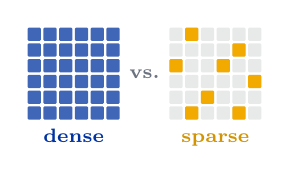
\begin{tikzpicture}[x=2.0mm,y=2.0mm]
  \foreach \r in {0,...,5} \foreach \c in {0,...,5} {
    \cell{\c}{\r}{navy!75}        % dense: every entry is a value
    \cell{\c+9}{\r}{ink!10}       % sparse: mostly zeros ...
  }
  \foreach \r/\c in {0/1,1/4,2/0,2/3,3/5,4/2,5/1,5/4}
    {\cell{\c+9}{\r}{gold}}       % ... and a few non-zeros
  \node[text=muted,font=\scriptsize\bfseries] at (7.42,-2.95) {vs.};
  \node[anchor=base,font=\scriptsize\bfseries,text=navy] at (2.92,-7.3) {dense};
  \node[anchor=base,font=\scriptsize\bfseries,text=gold!85!ink] at (11.92,-7.3) {sparse};
\end{tikzpicture}}

\begin{document}

%% ---------------------------------------------------------------------------
\maketitle
\note{(30 s) Two ways to beat the textbook triple loop. Part A keeps every operation but reorders them so the
caches are used well. Part B skips the zeros by storing only the non-zeros in CSR format. Everything is sequential
C, all kernels read the same inputs and give bit-identical results, and every configuration runs five times.}

%% ---------------------------------------------------------------------------
\begin{frame}{Dense Optimisations (Part A)}
\centering
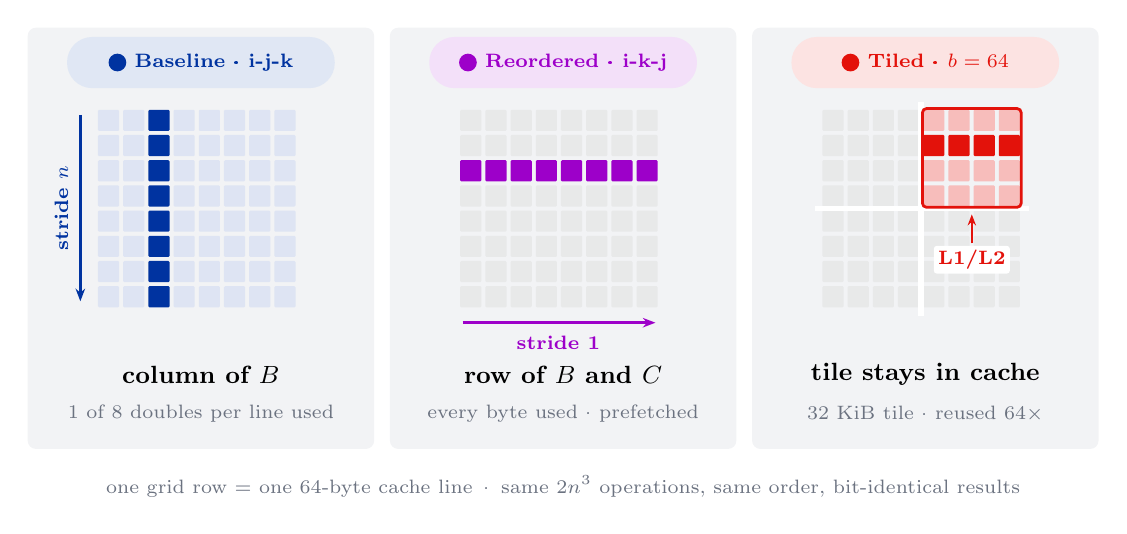
\begin{tikzpicture}
  \foreach \i in {1,2,3} \node[card] (c\i) at ({(\i-1)*4.6},0) {};

  % ---- 1: baseline, i-j-k: walks a COLUMN of B -----------------------------------
  \node[tag=navy] at ($(c1.north)+(0,-0.45)$) {\sdot{navy}\ Baseline \textperiodcentered\ i-j-k};
  \begin{scope}[shift={($(c1.north west)+(0.9,-1.05)$)},x=3.2mm,y=3.2mm]
    \foreach \r in {0,...,7} \foreach \c in {0,...,7} {
      \ifnum\c=2 \def\fc{navy}\else\def\fc{navy!13}\fi    % whole line loaded, one value used
      \cell{\c}{\r}{\fc}
    }
    \draw[-{Stealth[length=1.6mm]},navy,line width=1.1pt] (-0.7,-0.2) -- (-0.7,-7.6);
    \node[font=\scriptsize\bfseries,text=navy,rotate=90] at (-1.45,-3.9) {stride $n$};
  \end{scope}
  \node[font=\small\bfseries,align=center] at ($(c1.south)+(0,0.95)$) {column of $B$};
  \node[font=\scriptsize,text=muted,align=center] at ($(c1.south)+(0,0.45)$) {1 of 8 doubles per line used};

  % ---- 2: reordered, i-k-j: walks a ROW of B (and of C) ----------------------------
  \node[tag=purp] at ($(c2.north)+(0,-0.45)$) {\sdot{purp}\ Reordered \textperiodcentered\ i-k-j};
  \begin{scope}[shift={($(c2.north west)+(0.9,-1.05)$)},x=3.2mm,y=3.2mm]
    \foreach \r in {0,...,7} \foreach \c in {0,...,7} {
      \ifnum\r=2 \def\fc{purp}\else\def\fc{ink!10}\fi
      \cell{\c}{\r}{\fc}
    }
    \draw[-{Stealth[length=1.6mm]},purp,line width=1.1pt] (0.1,-8.45) -- (7.75,-8.45);
    \node[font=\scriptsize\bfseries,text=purp] at (3.9,-9.25) {stride 1};
  \end{scope}
  \node[font=\small\bfseries,align=center] at ($(c2.south)+(0,0.95)$) {row of $B$ and $C$};
  \node[font=\scriptsize,text=muted,align=center] at ($(c2.south)+(0,0.45)$) {every byte used \textperiodcentered\ prefetched};

  % ---- 3: tiled: one b x b tile stays in cache --------------------------------------
  \node[tag=brred] at ($(c3.north)+(0,-0.45)$) {\sdot{brred}\ Tiled \textperiodcentered\ $b=64$};
  \begin{scope}[shift={($(c3.north west)+(0.9,-1.05)$)},x=3.2mm,y=3.2mm]
    \foreach \r in {0,...,7} \foreach \c in {0,...,7} {
      \def\fc{ink!10}
      \ifnum\r<4 \ifnum\c>3 \def\fc{brred!28}\fi\fi       % the active tile
      \ifnum\r=1 \ifnum\c>3 \def\fc{brred}\fi\fi          % i-k-j inside the tile
      \cell{\c}{\r}{\fc}
    }
    \draw[white,line width=2pt] (3.92,0.3) -- (3.92,-8.2) (-0.3,-3.92) -- (8.2,-3.92);
    \draw[brred,line width=1pt,rounded corners=1.5pt] (3.97,0.05) rectangle (7.89,-3.87);
    \node[font=\scriptsize\bfseries,text=brred,fill=white,inner sep=1.5pt,rounded corners=1pt]
      at (5.93,-5.95) {L1/L2};
    \draw[-{Stealth[length=1.4mm]},brred,thick] (5.93,-5.3) -- (5.93,-4.15);
  \end{scope}
  \node[font=\small\bfseries,align=center] at ($(c3.south)+(0,0.95)$) {tile stays in cache};
  \node[font=\scriptsize,text=muted,align=center] at ($(c3.south)+(0,0.45)$) {32 KiB tile \textperiodcentered\ reused 64$\times$};

  % ---- what stays the same ------------------------------------------------------------
  \node[font=\scriptsize,text=muted] at (4.6,-3.15)
    {one grid row = one 64-byte cache line \,\textperiodcentered\, same $2n^3$ operations, same order, bit-identical results};
\end{tikzpicture}
\note{(1 min) Matrices are stored row by row, and memory arrives in 64-byte lines of eight doubles. The baseline's
inner loop walks down a column of B: every step loads a whole line and uses one double of it. Swapping the two
inner loops, i-k-j, walks along rows of B and C instead: stride one, every byte used, and the hardware prefetcher
sees the streams coming. Tiling goes one step further: it multiplies 64-by-64 blocks, 32 KiB each, so a block of B
is reused 64 times while it is still in L1 or L2, about 32 times less memory traffic. All three do exactly the same
operations in the same order, so the results are bit-identical; only the memory access pattern changes.}
\end{frame}

%% ---------------------------------------------------------------------------
\begin{frame}{Cache saturation at scale}
\begin{columns}[c]
\begin{column}{0.66\textwidth}
\centering
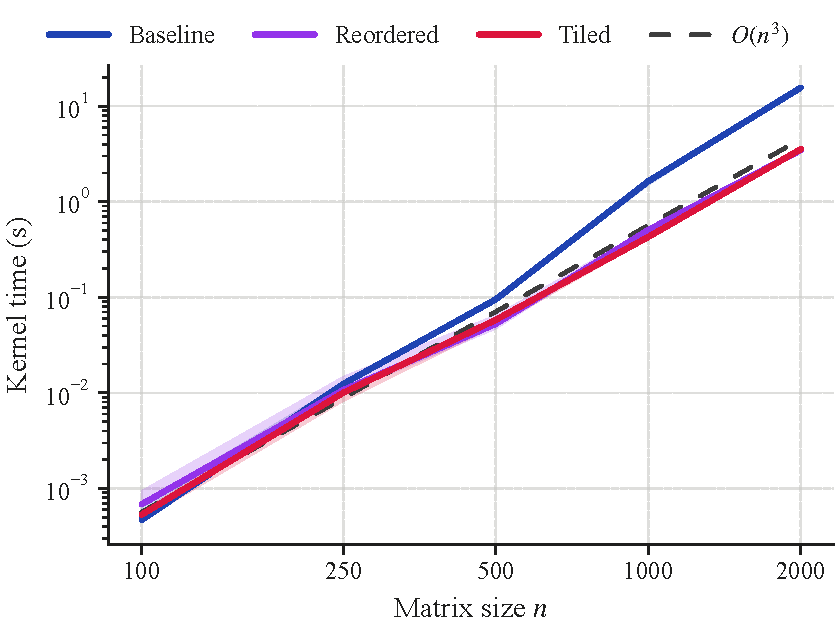
\includegraphics[height=0.76\textheight]{part_a_time_vs_size}\\[2pt]
{\scriptsize\muted{Median of 5 runs \textperiodcentered\ shaded: IQR \textperiodcentered\ log-log
\textperiodcentered\ dashed: $O(n^3)$ slope}}
\end{column}
\begin{column}{0.32\textwidth}
\bignum{4.5{\boldmath$\times$}}{faster at $n=2000$\\\muted{reordered \& tiled vs.\ baseline}}
\bignum{8\,MiB}{L3 filled by $B$\\\muted{at $n=1000$: baseline cost per op $\times 2$}}
\bignum{93\,MB}{peak memory\\\muted{identical for all three kernels}}
\end{column}
\end{columns}
\note{(1 min) Up to n = 250 everything fits in L2 and the three kernels are equal, within noise. From n = 500 the
optimised kernels pull away: at n = 2000 they take 3.5 seconds instead of 15.6, 4.5 times faster. The reason is the
L3 cache: at n = 1000, B alone is 7.6 MB, practically the whole 8 MiB L3, and the baseline's cost per multiply-add
doubles; at n = 2000, B is four times the L3. Reordered and tiled stay at about 0.43 ns per operation, so their time
grows exactly as n cubed (slope 3.0 against 3.7). Tiling does not beat reordering here: at -O2 the scalar loop, not
memory, is the bottleneck. And the speed-up is free: all three use the same 93 MB.}
\end{frame}

%% ---------------------------------------------------------------------------
\begin{frame}{Sparse Storage \& Fill-in (Part B)}
\centering
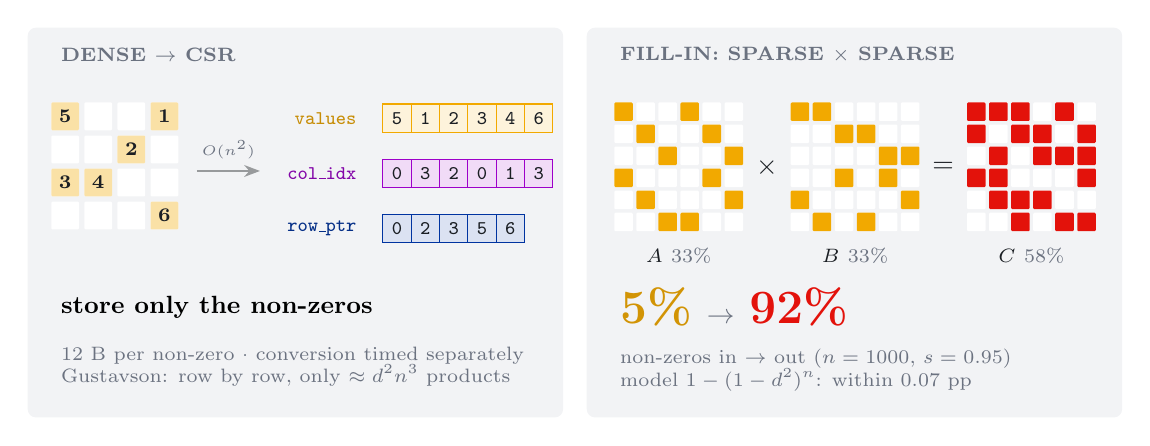
\begin{tikzpicture}
  % two cards (same visual language as the Part A slide)
  \fill[soft,rounded corners=3pt] (0,-1.75) rectangle (6.8,3.2);
  \fill[soft,rounded corners=3pt] (7.1,-1.75) rectangle (13.9,3.2);

  % ============ left card: dense -> CSR ==============================================
  \node[hdr] at (0.3,2.85) {DENSE $\to$ CSR};
  \begin{scope}[shift={(0.3,2.25)},x=4.2mm,y=4.2mm]
    \foreach \r in {0,...,3} \foreach \c in {0,...,3} {\cell{\c}{\r}{white}}
    \foreach \r/\c/\v in {0/0/5,0/3/1,1/2/2,2/0/3,2/1/4,3/3/6} {
      \cell{\c}{\r}{gold!35}
      \node[font=\scriptsize\bfseries,text=ink] at (\c+0.42,-\r-0.42) {\v};
    }
  \end{scope}
  \draw[flow] (2.15,1.38) -- (2.95,1.38);
  \node[font=\tiny\bfseries,text=muted] at (2.55,1.65) {$O(n^2)$};
  % the three CSR arrays
  \foreach \y/\name/\col/\vals in {
      2.05/values/gold/{5,1,2,3,4,6},
      1.35/col\_idx/purp/{0,3,2,0,1,3},
      0.65/row\_ptr/navy/{0,2,3,5,6}} {
    \node[anchor=east,font=\ttfamily\scriptsize,text=\col!80!ink] at (4.3,\y) {\name};
    \foreach \v [count=\k] in \vals
      \node[arr=\col] at ({4.33+\k*0.36},\y) {\v};
  }
  \node[font=\small\bfseries,anchor=west] at (0.3,-0.35) {store only the non-zeros};
  \node[font=\scriptsize,text=muted,anchor=west,align=left] at (0.3,-1.1)
    {12 B per non-zero \textperiodcentered\ conversion timed separately\\
     Gustavson: row by row, only $\approx d^2 n^3$ products};

  % ============ right card: fill-in ===================================================
  \node[hdr] at (7.4,2.85) {FILL-IN: SPARSE $\times$ SPARSE};
  \begin{scope}[shift={(7.45,2.25)},x=2.8mm,y=2.8mm]
    \foreach \r in {0,...,5} \foreach \c in {0,...,5}
      {\cell{\c}{\r}{white} \cell{\c+8}{\r}{white} \cell{\c+16}{\r}{white}}
    % A: two non-zeros per row
    \foreach \r/\c in {0/0,0/3,1/1,1/4,2/2,2/5,3/0,3/4,4/1,4/5,5/2,5/3} {\cell{\c}{\r}{gold}}
    % B: two non-zeros per row
    \foreach \r/\c in {0/0,0/1,1/2,1/3,2/4,2/5,3/2,3/4,4/0,4/5,5/1,5/3} {\cell{\c+8}{\r}{gold}}
    % C = A x B: row i of C is the union of the rows k of B selected by row i of A
    \foreach \r/\c in {0/0,0/1,0/2,0/4, 1/0,1/2,1/3,1/5, 2/1,2/3,2/4,2/5,
                       3/0,3/1,3/5, 4/1,4/2,4/3, 5/2,5/4,5/5} {\cell{\c+16}{\r}{brred}}
    \node[font=\bfseries,text=ink] at (6.92,-2.95) {$\times$};
    \node[font=\bfseries,text=ink] at (14.92,-2.95) {$=$};
    \foreach \x/\l/\p in {2.92/A/33,10.92/B/33,18.92/C/58}
      \node[font=\scriptsize\bfseries,text=ink] at (\x,-6.95) {$\l$ \muted{\textmd{\p\%}}};
  \end{scope}
  % the real numbers at n = 1000, s = 0.95
  \node[anchor=west] at (7.4,-0.35)
    {\fontsize{19}{21}\selectfont\bfseries\color{gold!85!ink}5\%%
     \;{\color{muted}\normalsize$\to$}\;%
     \color{brred}92\%};
  \node[font=\scriptsize,text=muted,anchor=west,align=left] at (7.4,-1.15)
    {non-zeros in $\to$ out ($n=1000$, $s=0.95$)\\
     model $1-(1-d^2)^n$: within 0.07 pp};
\end{tikzpicture}
\note{(1 min) CSR stores only the non-zeros: their values, their column indices, and where each row starts. That
costs 12 bytes per non-zero instead of 8 per entry, and converting a dense matrix costs n squared whatever the
sparsity, so we time it separately. Gustavson's algorithm then builds each row of C from the rows of B selected
by the non-zeros of A, the same row-wise order as i-k-j but skipping zeros, about d-squared n-cubed products.
The catch is fill-in: every non-zero of A spreads a whole row of B into C. With 95 percent zeros in the inputs,
the product still has 92 percent non-zeros, exactly what the probability model predicts.}
\end{frame}

%% ---------------------------------------------------------------------------
\begin{frame}{Where does sparse become viable?}
\begin{columns}[c]
\begin{column}{0.66\textwidth}
\centering
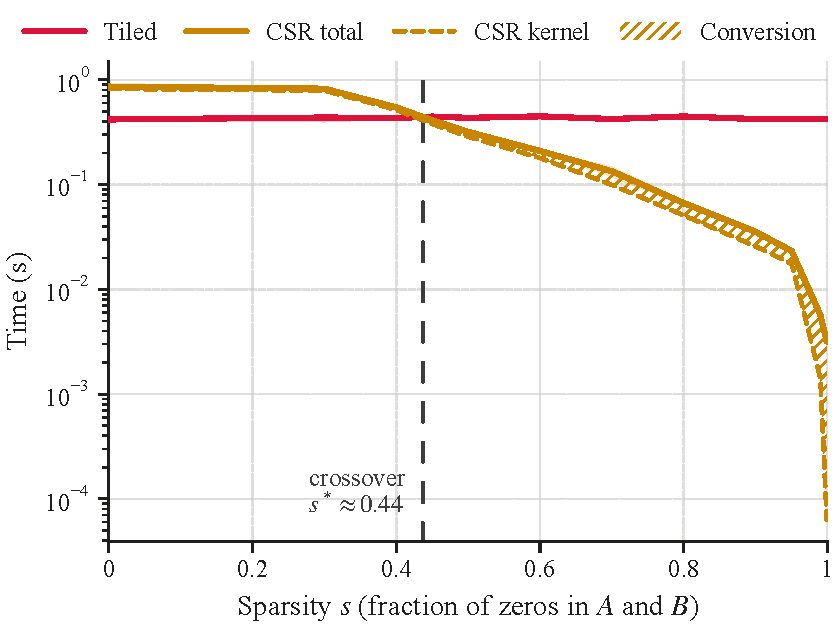
\includegraphics[height=0.70\textheight]{part_b_time_vs_sparsity}\\[2pt]
{\scriptsize\muted{$n=1000$ \textperiodcentered\ median of 5 runs \textperiodcentered\ CSR total = multiply + conversion (hatched)}}
\end{column}
\begin{column}{0.32\textwidth}
\bignum{44\%}{zeros: CSR beats tiled\\\muted{$s^* = 0.437$, with conversion}}
\bignum{97\%}{conversion $>$ multiply\\\muted{98\% of CSR time at 99.9\%}}
\bignum{132{\boldmath$\times$}}{faster at 99.9\% zeros\\\muted{including conversion}}
\end{column}
\end{columns}
{\scriptsize\muted{Scope: one machine (Ryzen AI 5 330, WSL 2), random sparsity, \texttt{gcc -O2} \textemdash\ not a universal ranking}}
\note{(1.5 min) The dense tiled kernel is flat at 0.43 seconds: zeros cost as much as any other value. CSR starts
twice as slow, but it overtakes tiled at 44 percent zeros, and the conversion barely moves that point (43 percent
without it). We compare with tiled on purpose: at zero sparsity CSR is already twice as fast as the baseline,
because Gustavson's row-wise traversal behaves like i-k-j, so comparing with the baseline would credit the loop
order to sparse storage. At high sparsity the picture flips: the multiplication shrinks with d squared but the
conversion stays n squared, so from 97 percent zeros converting costs more than multiplying, 98 percent of the time
at 99.9. Even so, CSR is 132 times faster there. All of this is for one machine and random sparsity patterns.}
\end{frame}

\end{document}
